\documentclass[10pt,twocolumn,letterpaper]{article}

\usepackage{cvpr}
\usepackage{times}
\usepackage{epsfig}
\usepackage{graphicx}
\usepackage{amsmath}
\usepackage{amssymb}
%\usepackage[backend=biber]{biblatex}
%\addbibresource{report\_submission.bib}

% Include other packages here, before hyperref.

% If you comment hyperref and then uncomment it, you should delete
% egpaper.aux before re-running latex.  (Or just hit 'q' on the first latex
% run, let it finish, and you should be clear).
\usepackage[breaklinks=true,colorlinks,bookmarks=false]{hyperref}

\cvprfinalcopy % *** Uncomment this line for the final submission

\def\cvprPaperID{****} % *** Enter the CVPR Paper ID here
\def\httilde{\mbox{\tt\raisebox{-.5ex}{\symbol{126}}}}

% Pages are numbered in submission mode, and unnumbered in camera-ready
\ifcvprfinal\pagestyle{empty}\fi
\begin{document}

%%%%%%%%% TITLE
\title{Project Report : CS 7643}

\author{Sakae Watanabe\\
Gatech\\
{\tt\small swatanabe30@gatech.edu}
% For a paper whose authors are all at the same institution,
% omit the following lines up until the closing ``}''.
% Additional authors and addresses can be added with ``\and'',
% just like the second author.
% To save space, use either the email address or home page, not both
\and
Ashish Narasimham\\
Gatech\\
{\tt\small anarasimham3@gatech.edu}
\and
Michael Walker\\
Gatech\\
{\tt\small mwalker311@gatech.edu}
}

\maketitle
%\thispagestyle{empty}

%%%%%%%%% ABSTRACT
\begin{abstract}
    We apply state-of-the-art Deep Learning approaches to the problem space of short-term trading, using daily market open/close/volume data to create time-series batches of sequences within the dataset. We take 3 different approaches: Spatio-Temporal Transformer (STT), Liquid Time-constant Network (LTCN), and Identity Recurrent Neural Network (IRNN); and attempt to extract signal from high-volatility public company stock movements in the healthcare space. Our results indicate that further investigation is required to create nuanced models that balance buying, selling, and holding inferences to achieve lower training loss. However we have been able to create a profitable trading strategy even with sub-optimal trading accuracy.

\end{abstract}

%%%%%%%%% BODY TEXT
\section{Introduction}

\subsection{Background} 

Simply, we attempted to generate profit on stock market historical data using deep learning methods. To reduce the scope, we focused on a basket of 5 stocks in the healthcare space that are publicly traded; we chose to focus on smaller companies, conjecturing that these are less influenced by algorithmic trading than the larger companies that have more visibility and are traded with higher volumes of shares exchanging hands. 
There are many large firms that have financial interests in optimizing profit algorithmically, so academic sharing of best practices isn’t the standard for the industry. There are a few papers published that survey modern techniques, but largely we sourced ideas from other industries and reapplied the tools to a new context while considering what might work well for time-series datasets.
Modern approaches generally have limitations across several dimensions. 1) They are better at classification than they are at regression. 2) They can predict near-term movements better than longer time horizons. 3) A myriad of data sources is required to accurately model stock movements - everything from political events and weather anomalies to X (formerly Twitter) posts and key individuals’ thoughts can provide strong signal for stock movements. 4) They need significant amounts of data to accurately distill patterns into weights.
If successful, beyond the immediate profits generated on the public trading markets this exploration would inform time-series deep learning approaches more broadly across industries. Real-time human vitals could be analyzed for anomalous adverse health events; automobile telemetry could be analyzed for part failure; and factory workers could be kept safe from industrial machinery malfunctions.


%-------------------------------------------------------------------------
%------------------------------------------------------------------------

\subsection{Data}

We gathered data from Yahoo! Finance’s daily stock data APIs to obtain historical pricing data for 5 different symbols\cite{yahoo_finance_api,yfinance}. A simple ETL pipeline was used to transform the data into usable input features. Four of the stock tickers were selected based on high volatility (more opportunity to outsmart the market if the stock goes further up and down), participation in the Healthcare space (interesting area that could be the next frontier for innovation), and small market cap (hopefully not as many competing algorithmic market participants). The final symbol SPX was selected to capture a broader signal to promote learning. Raw and processed data are stored in the GitHub repository.

\subsection{Dataset Properties}

The ticker data consists of columns date, open, high, low, close, adjusted close, and volume over the range 2020-10-18 to 2024-10-18. This daily ticker data can be used to train medium-term models on the order of days; intraday predictions would require data at 1- or 5-minute intervals.

\subsection{Training Splits}

The data was partitioned into training, validation, and testing sets as shown in Table~\ref{tab:trainingsplits}.

%\begin{table}
%    \begin{center}
%    \begin{tabular}{l|l|c|p{8cm}|}
%        & Train & Valid & Test \\
%        Start Date & 2020-10-18 & 2023-10-18 & 2024-04-18 \\
%    \end{tabular}
%    \caption{Training Splits}
%\label{tab:trainingsplits}
%\end{table}

\begin{table}
\begin{center}
    \begin{tabular}{|c|c|c|c|}
\hline
        & Train & Valid & Test \\
\hline
        Start Date & 2020-10-18 & 2023-10-18 & 2024-04-18 \\
\hline
        End Date & 2023-10-17 & 2024-04-17 & 2024-10-18 \\
\hline
        Time Span & 3 years & 6 mo & 6 mo \\
\hline
\end{tabular}
\end{center}
    \caption{Data splits and time frames.}
\label{tab:trainingsplits}
\end{table}

We labeled each row with one of three labels: buy, sell, or hold. The labels were a simple calculation based on the difference with the previous day: buy if it went up, sell if it went down, and hold if the delta is under a threshold.

    \subsection{Target Examples}
    Training examples were created by partitioning observations into windows of fixed-length $\tau$, where each window contained features $X_t = x_{t - \tau},..., x_t$. The target label for the window was computed based on next day returns.
% TODO <Some formal equation related to how target labels are created - can do an equation with cases here.> %y_t = \case based equation

    \subsection{Features}
A variety of technical indicators are commonly used in the enrichment of financial time-series data\cite{zou_survey,stock_charts}. The following features were added to the training data: 
    \begin{itemize}
        \item{Simple Moving Average (SMA): 10, 20, and 30 day}
        \item{Exponential Moving Average (EMA): 10, 20, and 30 day}
        \item{Relative Volume: 10, 20, and 30 day}
        \item{\%B: Computes the relative position of the current price within the 95\% confidence interval bands of SMA20}
        \item{Moving Average Convergence Divergence (MACD): An oscillation indicator using the 9, 12, and 26 day EMAs}
        \item{Relative Strength Index (RSI): An oscillation indicator grounded in the ratio of average gains to losses over a 14 day period. $RSI = 100 - \frac{100}{1 + RS}$, where $RS = \frac{AvgGain}{AvgLoss}$}
        \item{Momentum / Rate of Change: 10 day momentum. $Moment_t = price_t / price_{t-10} - 1$}
    \end{itemize}

Human traders that engage with markets on this timescale often use technical indicators such as these to make buy/sell decisions on their portfolio\cite{stock_charts}. Future areas of exploration would include combining these short-term signals with longer-term signals like metrics from the company’s balance sheet, sentiment analysis from earnings press releases, and social signals from the broader market participant pool.

    \section{Approach}
We took existing approaches in other industries and reapplied them to this new-to-us domain, taking a no-frills approach to data engineering, model training, and trading simulation in order to gain a deep (no pun intended) understanding and first-hand experience of the challenges in the space. We decided to structure the task as classification of next day movement - up, down or flat - rather than regression. Simply - we do not care by how much a stock will go up, we only care that it goes up so that we can buy it and subsequently sell when we predict it will reverse direction.

We applied the  Liquid Time-constant Network (LTCN), Spatio-Temporal Transformer (STT), and Identity RNN (IRNN) to the 5-stock dataset; we go into the model descriptions below.

    \begin{enumerate}
        \item{The Identity RNN (IRNN) is the simplest of our three models, leveraging the basic Recurrent Neural Network architecture. The name is such because this variant simplifies the initialization to an identity matrix (ones on the diagonal, zeros elsewhere) for the weights and 0’s for the biases to encourage the RNN to behave more like an LSTM. This works because when initializing to the identity matrix, the architecture tends toward an LSTM with the forget gate set to not decay the cell state at all. This is not equivalent to an LSTM but can stand in for one with comparative performance and a lot less parameters (4,000 learned parameters as tested), making for faster training cycles and lower inference latency.}
        \item{The Spatiotemporal Transformer (STT) leverages time2vec temporal encodings, a transformer-encoder stack, an LSTM decoder, and a fully connected classification module - 3.28M parameters as tested. The positional encoding utilized in the original transformer architecture only considers relative position within a context window. Temporal encodings extend upon this concept, allowing encodings to have relative importance across different context windows\cite{STT_Paper,time2vec,STLAT_sota,vaswani_attention_2023,BERT}.

STT combines temporal encoding with expanded multivariate time series data within the sequence. Financial time-series data consist of observations $x_t \in \mathbb{R}^d$, where $x_t$ represents the feature vector at time $t$. Rather than project $x_t$ to an arbitrary dimension, STT concatenates the temporal encoding $t2v \in \mathbb{R}^k$ with $x^i_t$, the $i$-th feature at time $t$ to produce intermediate embeddings. The expansion of the features combined with the concatenation of $t2v$ allows for more complex interactions across sequences and variables.

            The intermediate embedding $E_t \in \mathbb{R}^{d \times (k + 1)}$ is then passed through a dense embedding layer that projects to $\mathbb{R}^{d_{model}}$ that the transformer-encoder accepts.

Pretrained t2v Embedding
The t2v module of STT was pre-trained using a simple task of having a date at time $t$ predict the date at $t+1$ for the date range [1900-01-01, 2100-01-01]. This pre-training step provided additional stability during the primary model training and evaluation process. A more complex pre-training task may provide increased benefit, but was outside the scope of this experiment.
            Note: will help pass over once we get this in tex.}

        \item{Liquid Time-Constant Network (LTCN) \cite{hasani_liquid_2020} is a take on the Recurrent Neural Networks that is based on and inspired by biological neurons, specifically C. Elegens. Also known as a Liquid Neural Network (LNN), it uses a process to solve a series of Ordinary Differential Equations (ODEs) to solve problems in a way that allows the neural network to act in a spiking fashion, as well as being transparent in how it is performing its actions. LTCNs tend to require fewer resources than their deeper cousins - parameter count was 7,107 as tested - and work well with time series data, though they suffer from some of the same issues other RNNs suffer from, specifically vanishing gradients, especially with longer sequence data. Some solutions to these issues have been made, specifically Closed-form Continuous-time Neural nets \cite{CfC_LTC}, which seeks to reduce the number of Differential Equations down to 1 in an effort to better learn spatiotemporal tasks. Additionally, Liquid Structural State-Space Models (Liquid S4) were developed as an extension of the SSM in an effort to build a better performing model with spatiotemporal tasks \cite{hasani2022liquid}

        The main piece of the LTCN network is the use of ODE's, a system of equations, which depending on the implementation, could require an exponential number of discretized steps when simulated \cite{hasani_liquid_2020}. Instead, the paper that describes this model develops an ODE solver called a Fused Solver that fuses the explicit and implicit Euler methods. The Fused solver is defined by the following equation:
\begin{equation}
    x(t + \Delta t) = \frac{x(t) + \Delta t f(x(t), \textbf{I}(t), t, \theta)A}{1 + \Delta t(1/\tau _ f(x(t), \textbf{I}(t), t, \theta)}
\end{equation}

        Where $\textbf{I}(t)$ is the M-dimensional input, $\theta$ is the set of parameters, $\tau$
        is the time constant (this is "the parameter characteriziong the speed and the coupling sensitivity of an ODE" \cite{hasani_liquid_2020} the inverse of which is the membrane capacitance of our neuron \cite{LNN_Tutorial}), $A$ is a bias vector, $x(t)$ is our hidden value (which could be cellularized for a more LSTM experience, or have an LSTM tacked on as was present in the official library implementation \cite{NCP_Github}), $\Delta t$ is the step size, generally defined as $1 / L$ where $L$ = the number of layers or iterations we will run for our ODE solver, and finally $f(.)$ is a non-linear function. In our implementation, which we derived in part from the official library \cite{NCP_Github} and the following step by step tutorial \cite{LNN_Tutorial}, we added a way to switch up the nonlinearity beyond just a sigmoid or tanh, although most other nonlinearities did not train as well as the sigmoid or tanh.
        }.
    
    \end{enumerate}

\subsection{Evaluation Metrics}
Evaluation of classification performance focuses on True Positive (TP), True Negative (TN), and their false counterparts False Positive (FP) and False Negative (FN). The following classification based metrics were used to evaluate model performance:
Accuracy: The percentage of correctly predicted labels
 
\begin{equation} \label{eq:accuracy}
    Acc = \frac{TP + TN}{TP + TN + FP + FN}
\end{equation}

Matthews Correlation Coefficient (MCC): The MCC is commonly used when evaluating trade classifications for financial time-series data \cite{STT_Paper,STLAT_sota,zou_survey}. MCC is bound to the range [-1, 1], with +/- 1 indicating positively\/negatively correlated predictions respectively. MCC provides more robustness to class imbalance when compared to ACC.

\begin{equation} \label{eq:mcc}
    MCC = \frac{TP \times TN - FP \times FN}{TP + TN + FP + FN}
\end{equation}


\section{Experiments and Results}

Table~\ref{tab:general_results} contains the results we were able to achieve with best hyperparameter configuration per model class, with the additional constraint that we are using the same set of hyperparameters for all ticker symbols to promote generalization across market data. This was set up as a 3-class classification task - sell, hold, or buy.

\begin{table}
\begin{center}
    \resizebox{\columnwidth}{!}{%
    \begin{tabular}{|c|c|c|c|c|}
\hline
        \multicolumn{5}{|c|}{Accuracy, MCC} \\
\hline
        & ATNF & BIVI & CYCC & VTAK \\
\hline
        RNN & 0.378, .0837 & .511, .0768 & .543, .0782 & .276, .046 \\
\hline
        Transformer & .37, .0446 & .433, .0815 & .433, .0578 & .323, -.0668 \\
\hline
        LNN & .52, 0 & .504, 0 & .535, 0 & .496, 0 \\
\hline
\end{tabular}%
    }
\end{center}
\caption{Data splits and time frames.}
\label{tab:general_results}
\end{table}

Although we were initially disappointed by the~50\% test accuracy across all three models, they generally ended with gains across the 6-month test window when put into simulation. This indicates that although they were noisy in their inferences, the training data enabled them to identify the key inflection points of the chart as they were happening. Some models learned to be very selective when buying and liberal when selling, in effect identifying entry points with very high confidence of a positive movement and then selling after losing some of that confidence.  <should we more formally lay this out in a table? Class distribution per model on test data>

\begin{table}
\begin{center}
\resizebox{\columnwidth}{!}{%
\begin{tabular}{|c|c|c|c|}
\hline
\textbf{Model} & \textbf{Avg. Epoch Time} & \textbf{Avg. Train Time} & \textbf{Avg. Valid Time} \\ \hline
RNN           & 0.1153                      & 0.1113                         & 0.2171                           \\ \hline
Transformer   & 0.4647                      & 0.4574                         & 1.1957                           \\ \hline
LNN           & 3.3816                      & 3.3173                         & 3.2862                           \\ \hline
\end{tabular}%
}
\end{center}
\caption{Time in seconds of each models' Average Epoch, Training, and Validation performance}
\label{tab:metrics}
\end{table}

\subsection{Shared Hyperparameters}

We found that each stock will be predicted optimally by a specific set of hyperparameters; it may not be the case that a single set of hyperparameters should work well across the board, given the nuances of each symbol’s movements. However that single configuration can give a great place to start from when incorporating a new symbol into one’s trading portfolio.
One other note - the transformer leverages about 1000x the parameter count as the other two models do. This begs the question, is it worth it? The results paint a mixed picture, which is not a clear signal towards the Transformer-based model. Under the construct of using a single hyperparameter set, we don’t have an answer. However future research could investigate individually tuning per symbol, perhaps allowing a best algorithm to emerge there.

The experiments below are ablation studies testing two hypotheses we had; we focused on the \$BIVI symbol and stock ticker for these experiments.


\begin{figure*}[ht!]
    \centering
    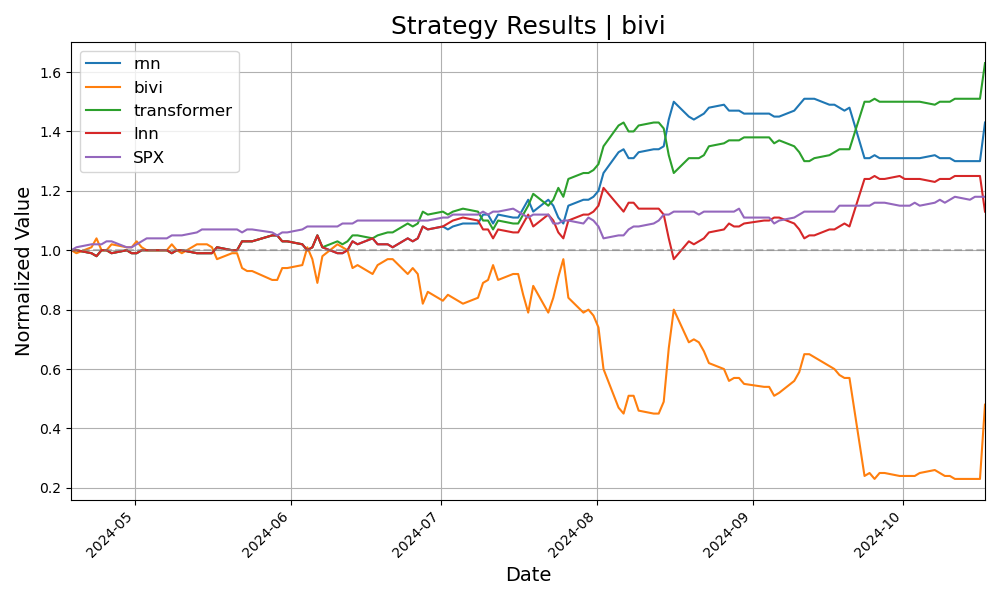
\includegraphics[width=0.48\textwidth]{../figures/simulation_results_all_models_bivi_config_loss_ce.yml.png}
    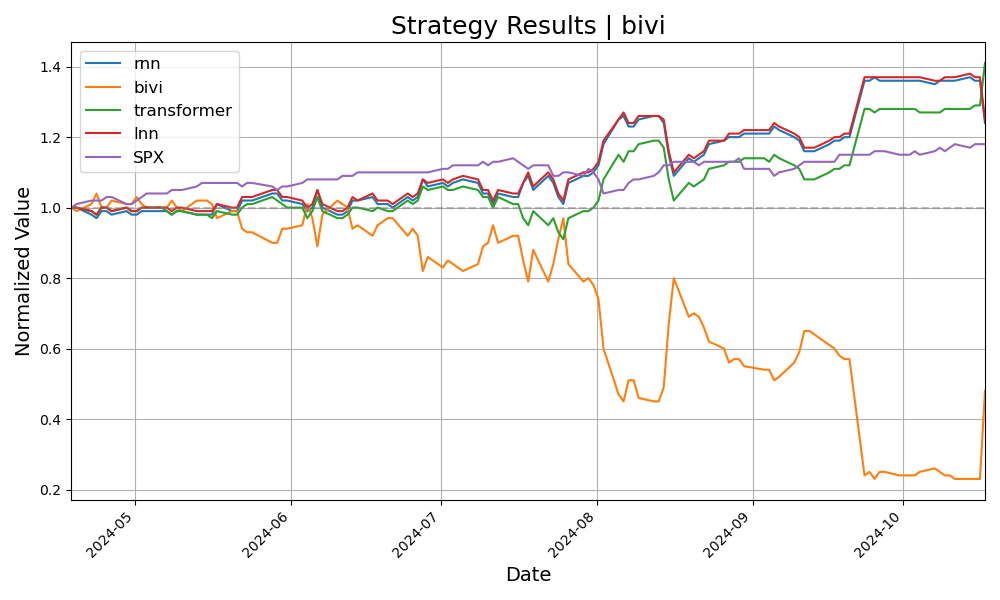
\includegraphics[width=0.48\textwidth]{../figures/simulation_results_all_models_bivi_config_loss_cbfocal.yml.png} 
    \caption{Comparison of results using both CE and CB loss functions for the symbol \$BIVI. \emph{Left}: Simulation results comparison for CE. \emph{Right}: Simulation results using class balanced focal loss (CB).}
    \label{fig:ceVsCbLoss}
\end{figure*}

\subsection{Optimizers and Loss Functions}

The first ablation study we were interested in was testing different loss functions due to the distribution of the source data. Since the label distribution is imbalanced (24\%, 37\%, 35\%, and 42\% buy labels), class-balanced focal loss could help to appropriately weight the dataset\cite{cb_focal}. We contrasted this with vanilla Cross Entropy Loss (CE).

Both the RNN and Transformer perform better with the standard cross-entropy loss, but the LTCN performs best with class-balanced focal loss. For the tested symbol, the Transformer had the best overall strategy test outcome. Both the RNN and the STT (containing an LSTM) do better with CE loss; an explanation for this could be that the models should not be weighting the imbalanced classes higher, as they might learn e.g. a buy probability that is too high for that particular situation. It is interesting that the LTCN has almost the same strategy across the two losses, it is just shifted up a little bit. This indicates that the class balancing that the loss function applies is scaling the strategy's profit in a beneficial way.

\subsection{Adding Additional Data with Pretraining}

Another idea we validated was that signal from a broader selection of market data will benefit learning for the target dataset and ticker. We tested including other tickers from our dataset in a pre-training phase. We included all tickers except the target symbol in the pre-training phase, running the ablation study by varying the percentage of epochs spent training on the all-but-target-symbol dataset versus fine-tuning on the target symbol. For fine-tuning, we introduced another parameter to step down the learning rate and held that constant per model across this study, using the best value found per model.  Results are presented below.

\begin{figure*}[ht!]
    \centering
    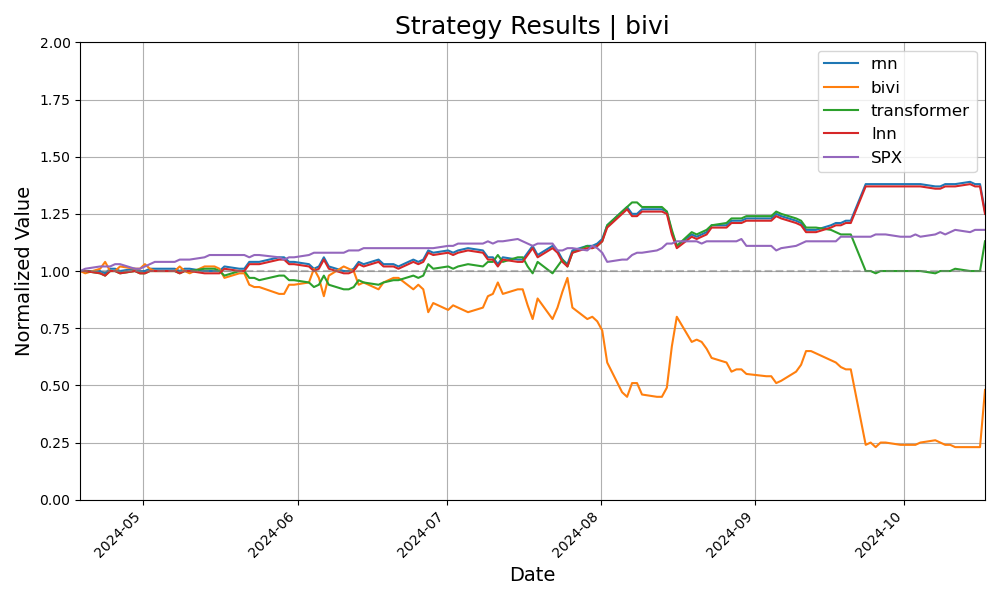
\includegraphics[width=0.48\textwidth]{../figures/simulation_results_all_models_bivi_config_target_split_75_regenerated_anarasimham.yml.png}
    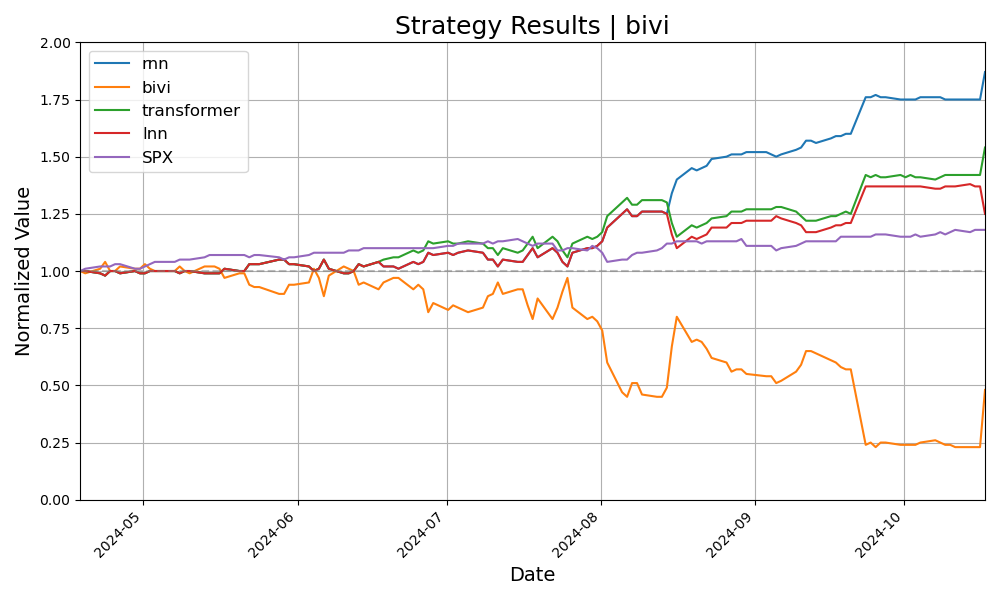
\includegraphics[width=0.48\textwidth]{../figures/simulation_results_all_models_bivi_config_target_split_99.yml.png} 
    \caption{Comparison of pretraining/fine-tuning ablation; 75\% (left) and 99\% (right) pretraining selected for further visualization here.}
    \label{fig:pretrainingsplits}
\end{figure*}

The RNN performs well across both the 75\% and 99\% splits. Not shown here is the 25\% split, where the RNN performs at the top of the group of models as well but lower from an absolute profitability standpoint. The RNN seems to learn well from pretraining data, especially when the target symbol is excluded. We tried experiments including the target symbol in pretraining data, and that significantly and adversely affected the RNN output. In those cases, this may be due to the RNN overfitting the target symbol training data and therefore losing accuracy on the test set. The Transformer and LTCN do not seem to be as sensitive to this type of data, and this is perhaps due to the increased dimensionality of those models. Future research might focus on gathering more data to feed these other two model types to understand if that improves their pretraining outcomes as well.

\section{Conclusion}

We conjectured that the Spatio-Temporal Transformer with its many parameters would have higher representational power and therefore be able to extract much higher returns from the market for the target symbols; we were proven wrong there. The model that came back with the most positive surprise was also the simplest - the RNN. The RNN, with the fewest number of parameters out of the three, excelled at predicting a subset of the symbols that we tested. It did not perform well on all of them, but given the single hyperparameter constraint this was not too much of a surprise. Out of the box and given a few interesting technical indicators extracted from the world of trading, these models are able to identify strong signal from the data and use that to become profitable, at least for the test sets defined in this set of experiments.

Looking forward, we’d look at testing these models further to validate their generalizability across industries, instruments, etc. - commodities, futures, and cryptocurrency are all interesting areas with their own opportunities and challenges. In terms of engineering work, additional intelligence can be added both when creating the labels for the dataset and when running the simulation to improve profitability of the strategy. Execution control, e.g. selling when at a 10\% loss, could probably also improve profitability but outside of the Deep Learning walls of this experiment.


%-------------------------------------------------------------------------
\clearpage
\section{Work Division}

\begin{table*}
\begin{tabular}{|l|c|p{8cm}|}
\hline
Student Name & Contributed Aspects & Details \\
\hline\hline
Sakae Watanabe & Implementation, Experimentation & Data \& feature engineering; training base code; STT model build/tune; trading simulation\\
Ashish Narasimham & Implementation, Paper Writing & Dataset sourcing; training code generalization; pre-training feature; RNN model build/tune; paper writing \\
Michael Walker & Implementation, Experimentation & Refactor code and configuration for reusability; experiment setup; LNN model build/tune \\
\hline
\end{tabular}
\caption{Contributions of team members.}
\label{tab:contributions}
\end{table*}

The team felt that team members’ contributions met a minimum bar, and no group member was absent from the project work. Sakae wrote the majority of the framework code around the models - data engineering, feature engineering, experimentation, and trading simulation; Ashish and Michael contributed to refactors of that code for generalization and reusability. We each contributed our own model development and tuning, and all had ideas for experimentation/analysis.


%%%%%%%%% REFERENCES
\bibliographystyle{unsrt}
\bibliography{egbib}

\end{document}
